\section{Résultats obtenus}
Les résultats obtenus au terme du projet ont été globalement satisfaisants, répondant aux objectifs fixés. La reprise des données, et en particulier des \textbf{measure\_requests}, a été réalisée garantissant la conformité aux spécifications du client.
Le processus global, incluant l’extraction avec l’esquilo, la transformation via l’extracteur, et les validations par tests automatisés, a permis de livrer des données propres et prêtes à être utilisées dans le système Padoa. 

Le client SSTI03 a commencé à utiliser le logiciel padoa le 26 November 2024. Jusqu'à présent, aucun retour sur la reprise des examens complémentaires n'a été fait. Ce qui montre que le client est globalement satisfait de la migration des données. 

\begin{figure}[h!]
    \centering
    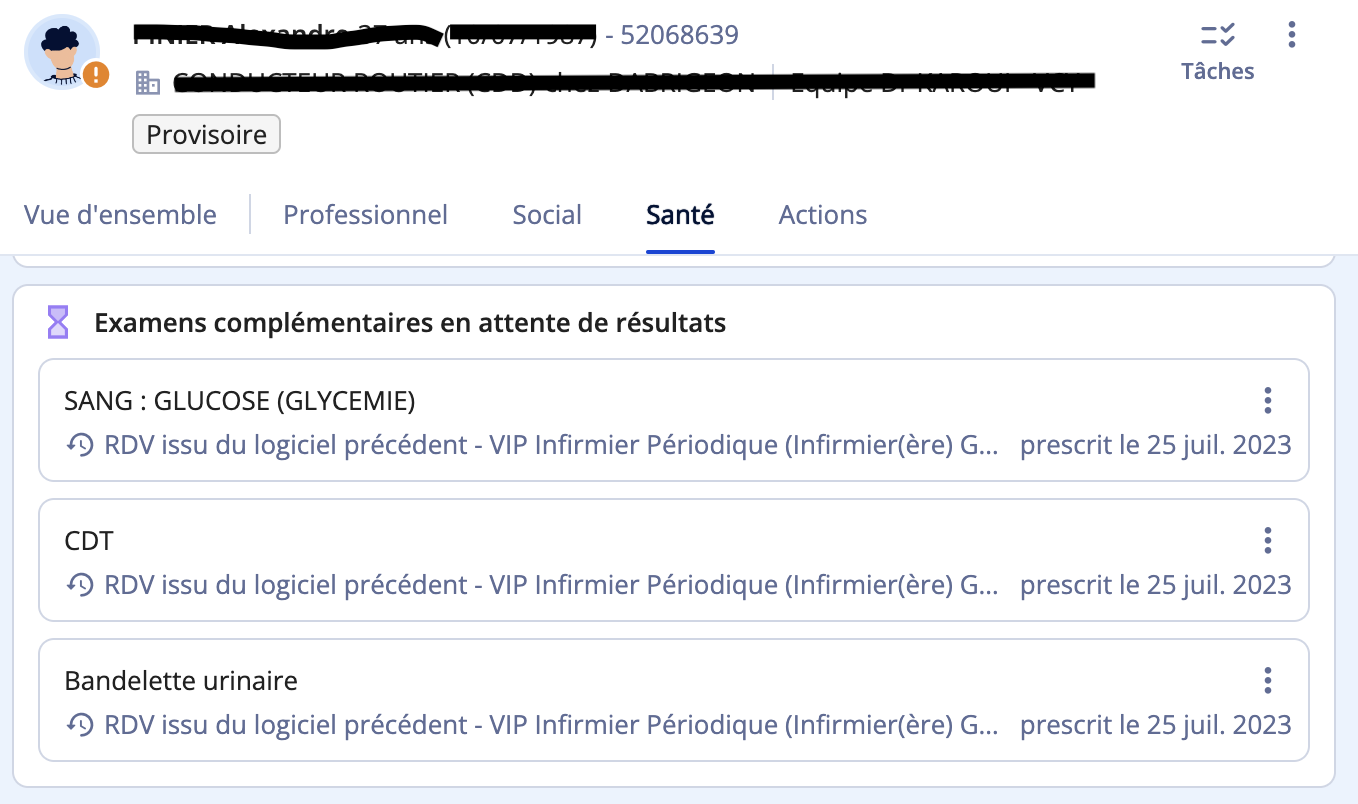
\includegraphics[width=0.7\textwidth]{4_attachments/figures/padoa_exam.png} % Remplacez "image.png" par votre fichier
    \caption{Examens complémentaires en attente de résultat sur padoa}
    \label{fig:upside_down}
\end{figure}

\begin{figure}[h!]
    \centering
    % Première image (en haut)
    \begin{subfigure}{\textwidth}
        \centering
        
\includegraphics[width=0.7\textwidth]{4_attachments/figures/prev_bef.png} % Remplacez "image1.png"
        \caption{Sur préventiel}
        \label{fig:image1}
    \end{subfigure}
    
    \vspace{1cm} % Espacement entre les images
    
    % Deuxième image (en bas)
    \begin{subfigure}{\textwidth}
        \centering
        
\includegraphics[width=0.7\textwidth]{4_attachments/figures/padoa_bef.png} % Remplacez "image2.png"
        \caption{Sur padoa}
        \label{fig:image2}
    \end{subfigure}
    
    \caption{Examens complémentaires en attente de résultat avant 31 Octobre 2022}
    \label{fig:stacked_images}
\end{figure}

\begin{figure}[h!]
    \centering
    % Première image (en haut)
    \begin{subfigure}{\textwidth}
        \centering
        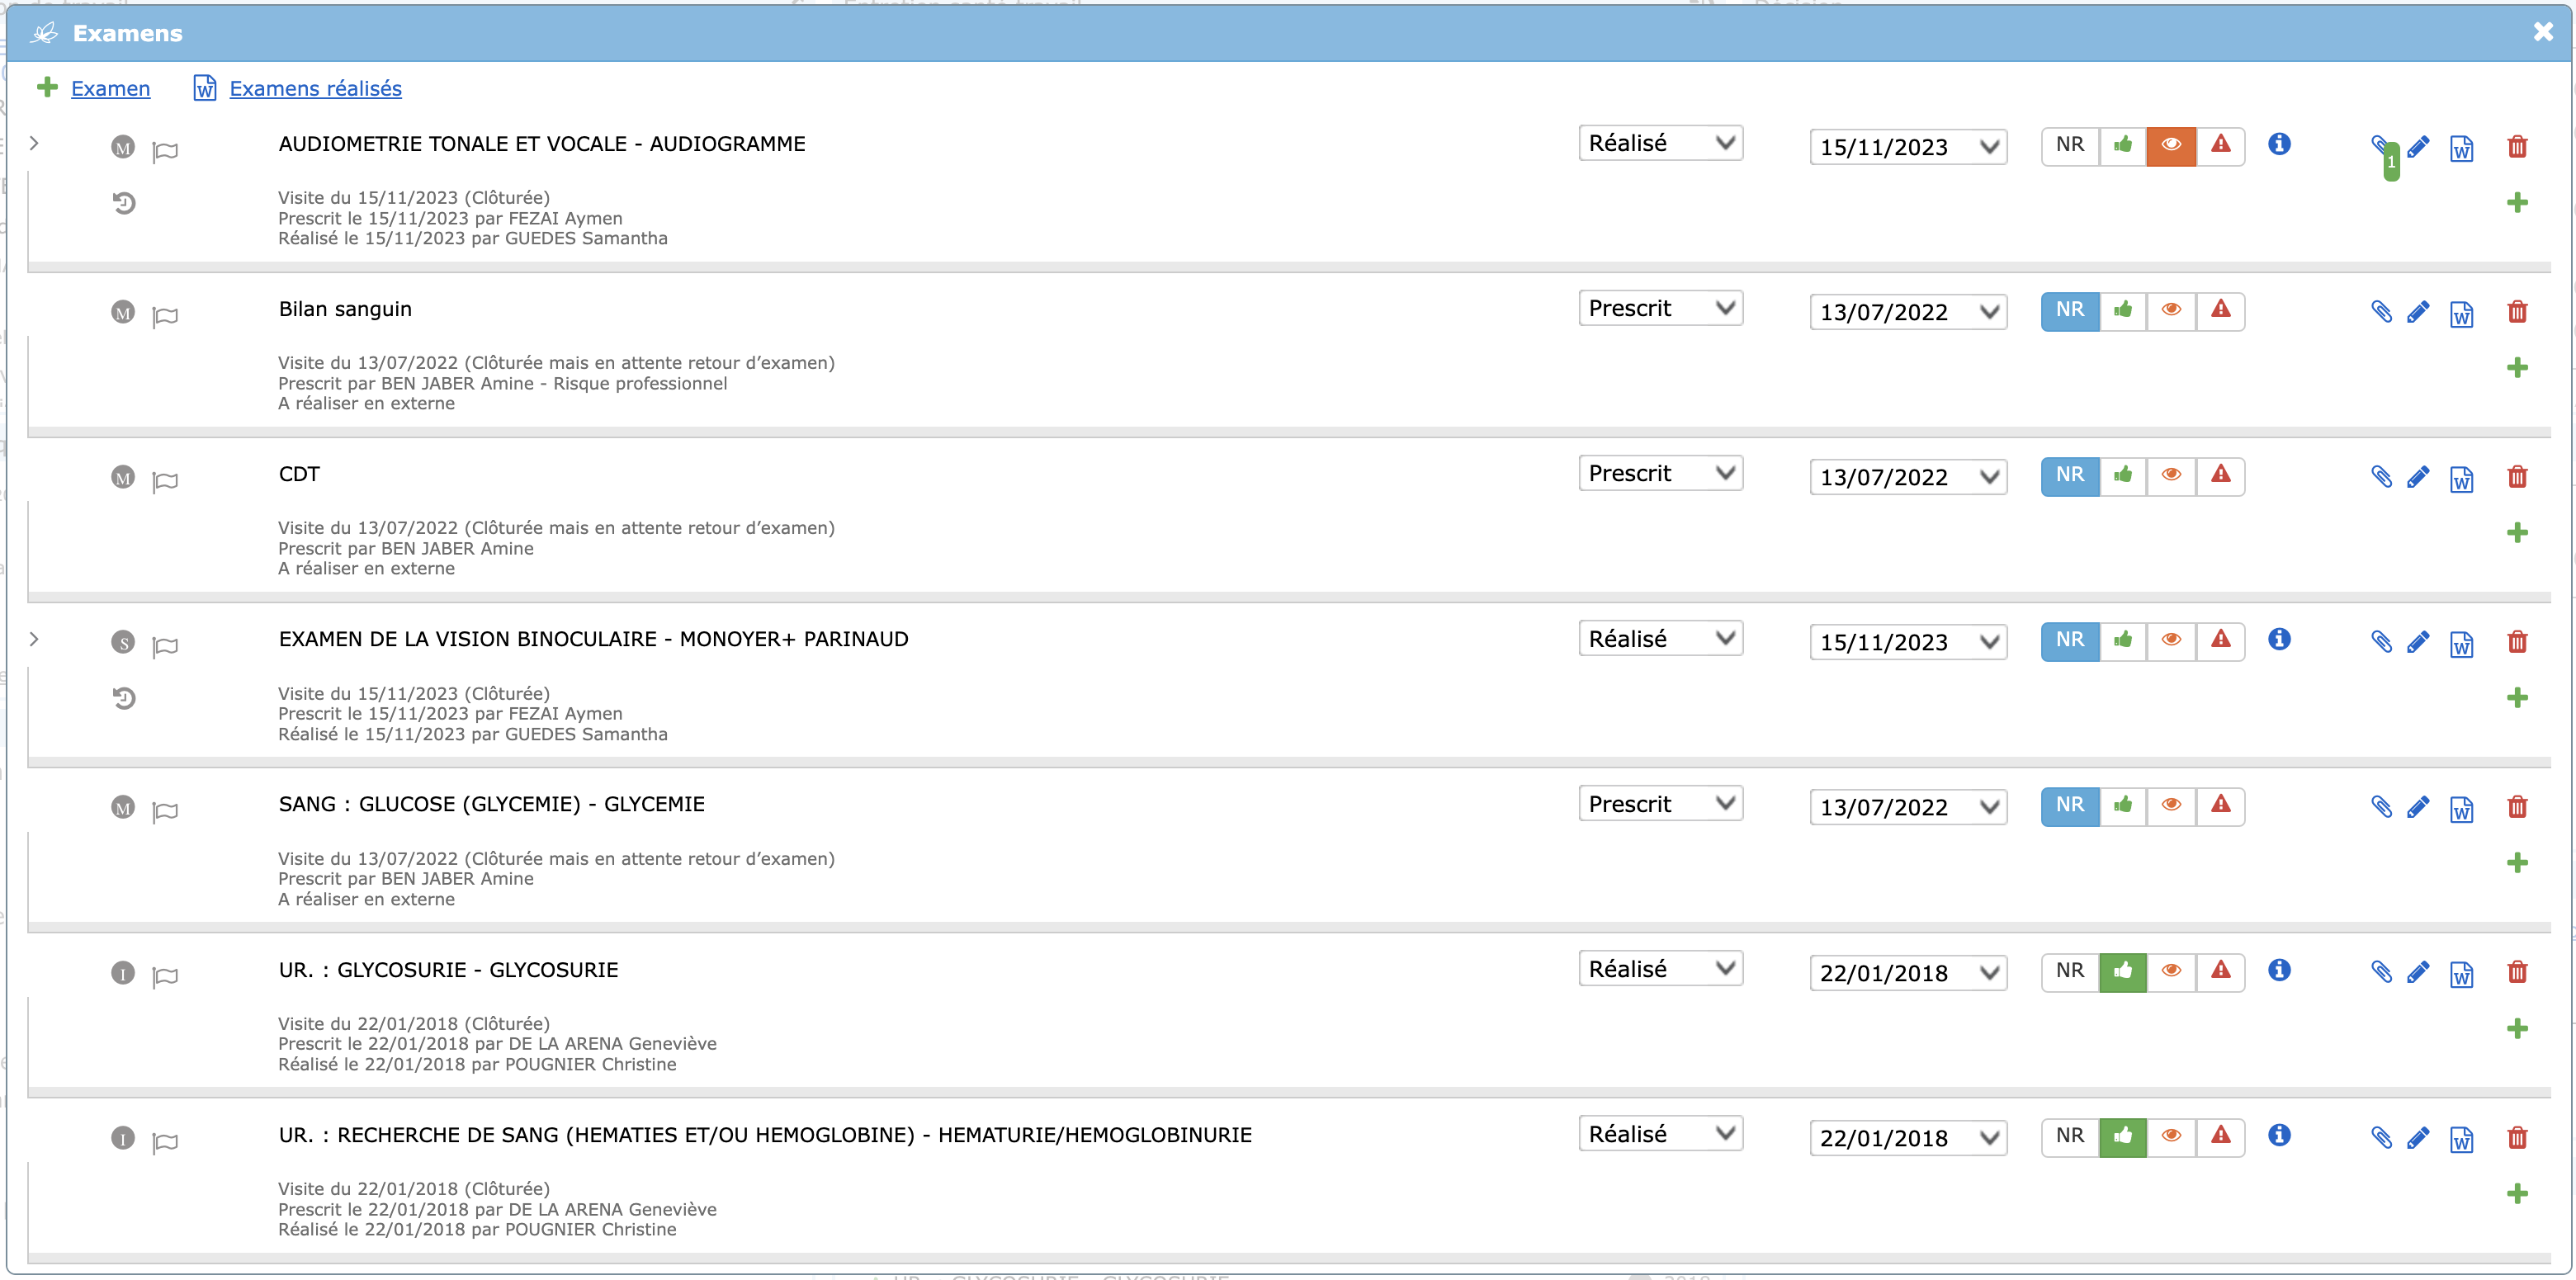
\includegraphics[width=0.7\textwidth]{4_attachments/figures/prev_ex_full.png} % Remplacez "image1.png"
        \caption{Sur préventiel}
        \label{fig:image1}
    \end{subfigure}
    
    \vspace{1cm} % Espacement entre les images
    
    % Deuxième image (en bas)
    \begin{subfigure}{\textwidth}
        \centering
        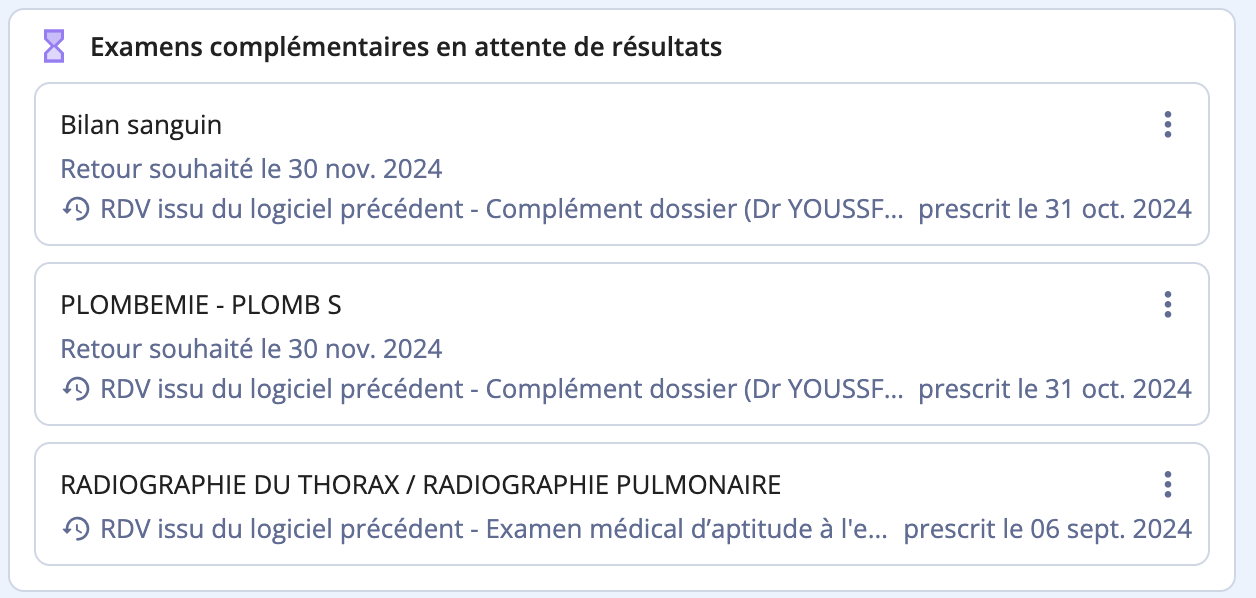
\includegraphics[width=0.7\textwidth]{4_attachments/figures/padoa_ex_full.png} % Remplacez "image2.png"
        \caption{Sur padoa}
        \label{fig:image2}
    \end{subfigure}
    
    \caption{Reprise des examens complémentaires en attente de résultat}
    \label{fig:stacked_images}
\end{figure}


\clearpage